\section{Introduction}


%%%%%%%%%%%%%%%%%%%%%%%%%%%%%%%%%%%%%%%%%%%%%%%%%%%%%%%%%%%%%%%%%%%%%%%%%%%%%%%%%%%%%%%%%%%%%%%%%%%% 
\begin{frame}{Computation Demands}
\begin{columns}[c]
  \begin{column}{0.5\textwidth}
    Over the last 15 years, the required \textbf{training computations have been approximately doubled every 6 months.}

    \vspace{20pt}

    This indicates the \textbf{synergistic advances achieved} in both deep learning
    \textbf{methodologies} and \textbf{hardware}
    capabilities.\footnotemark
  \end{column}
  \begin{column}{0.5\textwidth}
    \begin{center}
      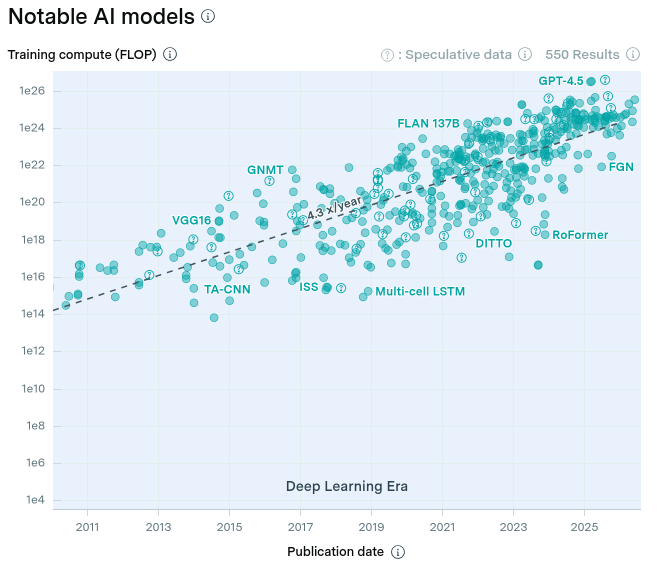
\includegraphics[width=\linewidth]{sections/0_intro/imgs/epoch-ml-trends-2.png}
    \end{center}
  \end{column}
\end{columns}
\footnotetext{\textbf{Source:} Sevilla, Jaime, et al. "Compute trends
  across three eras of machine learning." 2022 International Joint Conference on
  Neural Networks (IJCNN). IEEE, 2022. (https://epoch.ai/blog/compute-trends)}
\end{frame}

%%%%%%%%%%%%%%%%%%%%%%%%%%%%%%%%%%%%%%%%%%%%%%%%%%%%%%%%%%%%%%%%%%%%%%%%%%%%%%%%%%%%%%%%%%%%%%%%%%%% 

\begin{frame}{Hardware Accelerator}
\begin{itemize}
    \item \textbf{Pushing the boundaries of available hardware}
    \item Reveals the need to \textbf{shift towards specialized hardware}
\end{itemize} \vspace{15pt}

    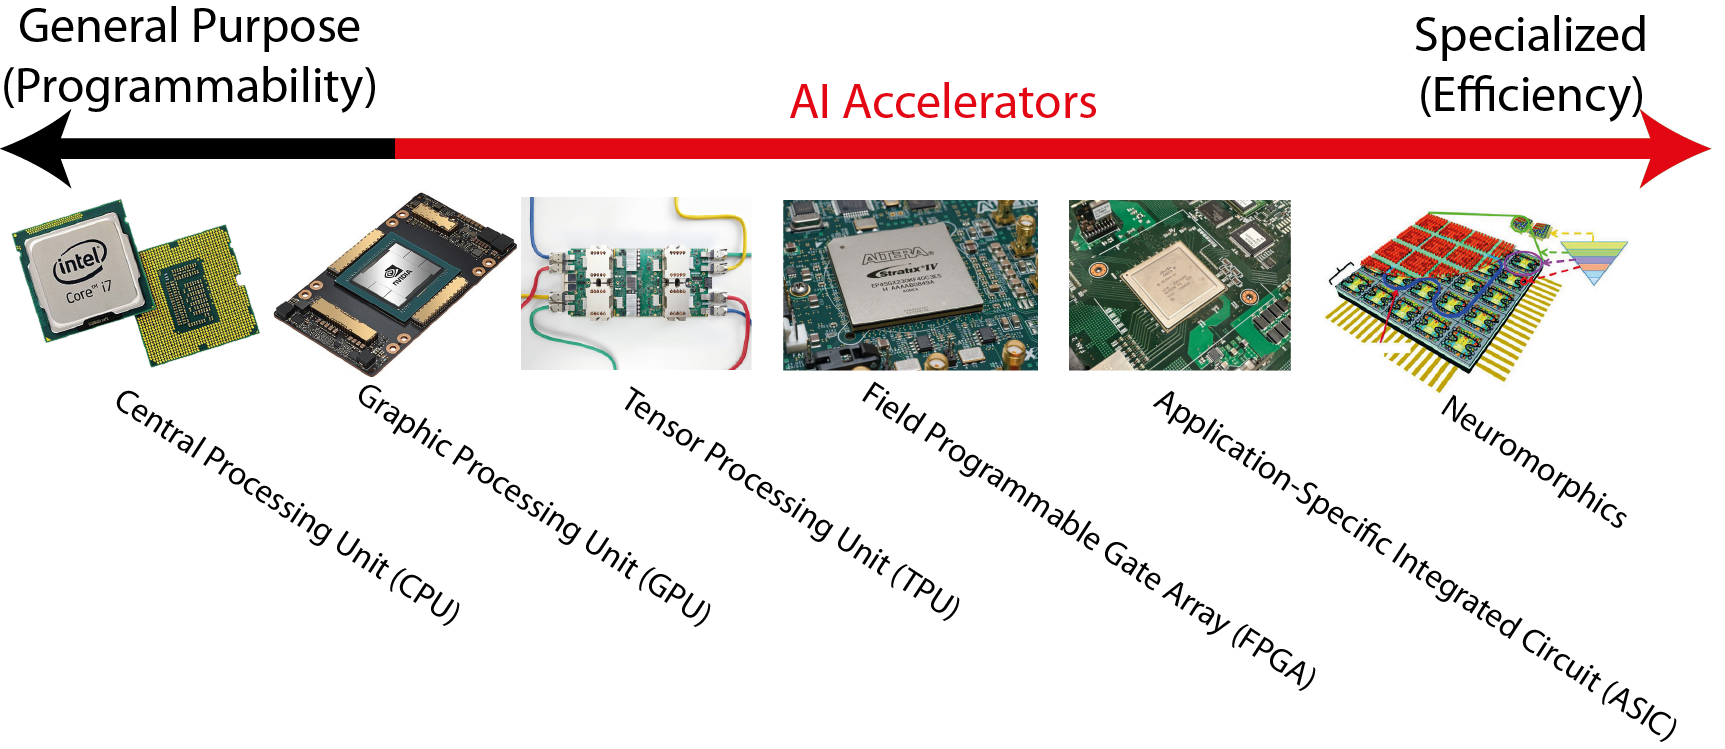
\includegraphics[width=0.9\linewidth]{sections/0_intro/imgs/intro_phd.png}
\end{frame}

%%%%%%%%%%%%%%%%%%%%%%%%%%%%%%%%%%%%%%%%%%%%%%%%%%%%%%%%%%%%%%%%%%%%%%%%%%%%%%%%%%%%%%%%%%%%%%%%%%%% 


\begin{frame}{Integrated Silicon Photonics}
  \textbf{Photonic neurons encode signal using light},  which are then manipulated to provide functionality in neurons. \vspace{-5pt}
  % rather than electric quantities,
  % Providing a great potential to be used in DL accelerators due to:
  \begin{center}
    \begin{figure}
        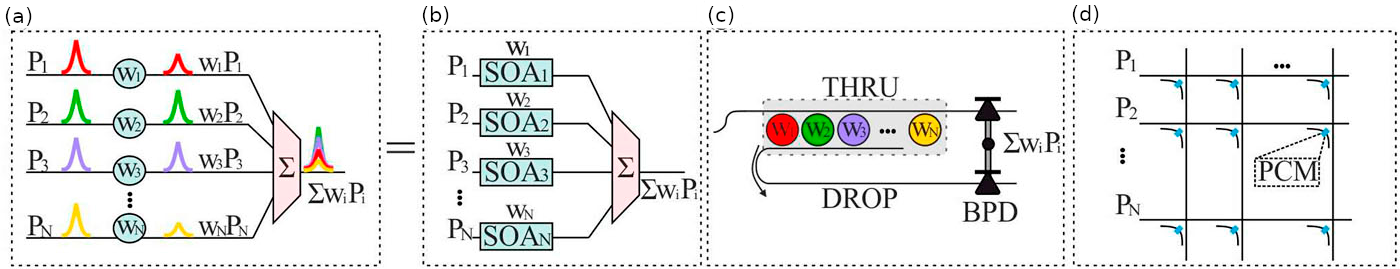
\includegraphics[width=\linewidth]{sections/0_intro/imgs/apl_incoherent.png}
        \caption{Indicative layouts adopt the incoherent
          concept.\footnote{\textbf{Source:} Tsakyridis, A., Moralis-Pegios, M., Giamougiannis, G., Kirtas, M., Passalis, N., Tefas, A. and Pleros, N., 2024. Photonic neural networks and optics-informed deep learning fundamentals. APL photonics, 9(1).} \vspace{-5pt}}
    \end{figure}
  \end{center}
  A majority of currently available \textbf{photonic architectures rely on incoherent layouts}.
\end{frame}

%%%%%%%%%%%%%%%%%%%%%%%%%%%%%%%%%%%%%%%%%%%%%%%%%%%%%%%%%%%%%%%%%%%%%%%%%%%%%%%%%%%%%%%%%%%%%%%%%%%%
\begin{frame}{Incoherent Photonics \& The Sign Problem}

\begin{columns}[T]

%% ── LEFT COLUMN ─────────────────────────────────────────────
\begin{column}{0.46\textwidth}
  \vspace{0.1em}
  In incoherent photonics the  optical signals are converted into
  \textbf{power signals} during the activation stage.

    % ── wave picture ────────────────────────────────────────────
  \begin{center}
  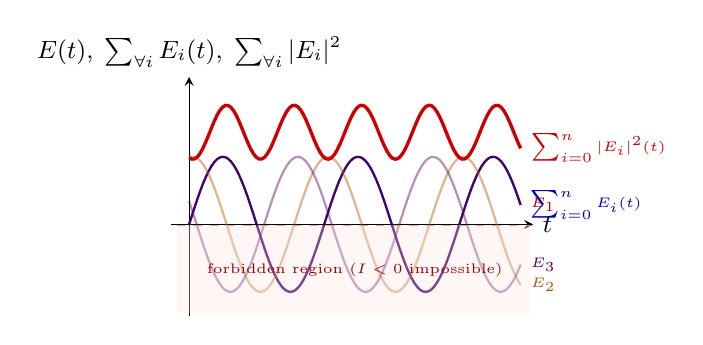
\begin{tikzpicture}[scale=0.78, >=stealth]

    %% axes
    \draw[->] (-0.3,0) -- (5.6,0) node[right,font=\small] {$t$};
    \draw[->] (0,-1.5) -- (0, 2.4) node[above,font=\small] {$E(t),\; \sum_{\forall i}E_i(t),\; \sum_{\forall i}|E_{i}|^2$};

    %% electric field  E(t) = sin
    \draw[blue!70!black, thick, domain=0:5.4, samples=120]
      plot (\x, {1.1*sin(360*\x/2.2)})
      node[right, font=\tiny, blue!70!black] {$\sum_{i=0}^{n}E_{i}(t)$};

    %% incoherent intensities — three sources with random phases
    \draw[red!70!black, thick, opacity=0.4, domain=0:5.4, samples=120]
      plot (\x, {1.1*(sin(360*\x/2.2))})
      node[right, font=\tiny, red!70!black, opacity=1] {$E_1$};
    \draw[orange!70!black, thick, opacity=0.44, domain=0:5.4, samples=120]
      plot (\x, {1.1*(sin(360*\x/2.2+80))})
      node[right, font=\tiny, orange!70!black, opacity=1] {$E_2$};
    \draw[violet!70!black, thick, opacity=0.44, domain=0:5.4, samples=120]
      plot (\x, {1.1*(sin(360*\x/2.2+160))})
      node[right, font=\tiny, violet!70!black, opacity=1] {$E_3$};

    %% I_total = Σ|E_i|²  (incoherent: no cross-terms)
    \draw[red!80!black, very thick, domain=0:5.4, samples=120]
      plot (\x, {1* ((sin(360*\x/2.2))^2+(sin(360*\x/2.2+80))^2+(sin(360*\x/2.2+160))^2)})
      node[right, font=\tiny, red!80!black] {$\sum_{i=0}^{n}|E_{i}|^{2}(t)$};

    %% forbidden zone label
    \fill[red!12, opacity=0.3] (-0.2,-1.45) rectangle (5.55,-0.02);
    \draw[red!40, dashed] (-0.2,-0.02) -- (5.55,-0.02);
    \node[font=\tiny, red!60!black] at (2.7,-0.75)
      {forbidden region ($I < 0$ impossible)};

    %% annotation arrows
    % \draw[->, gray, thin] (1.35,1.45)
    %   to[bend left=20] node[midway, right, font=\tiny]{$\scriptstyle |E|^2$}
    %   (1.55,0.95);
    \end{tikzpicture}
  \end{center}

  \vspace{1.2em}
\end{column}

\hfill
%% ── RIGHT COLUMN ────────────────────────────────────────────
\begin{column}{0.50\textwidth}
  An electromagnetic wave propagating in a medium has an electric field:
  \[E(r, t) = A e^{i(kr - \omega t)}\]

  A photodetector measures the optical intensity:
  \[
    I = \tfrac{1}{2}\,\varepsilon_0 c\,|E|^2 \;\geq\; 0
  \]
  The generated photocurrent given by
  \[
    i_{\mathrm{ph}} = \mathcal{R}\cdot P = \mathcal{R}
    \int_{\!\mathcal{A}} I\,\mathrm{d}A \;\geq\; 0
  \]


  % \vspace{0.3em}
  % \centering
  % \begin{tabular}{@{}lcc@{}}
  %   \hline
  %   \textbf{Quantity} & \textbf{Range} & \textbf{Signed?} \\
  %   \hline
  %   Field $E$          & $\mathbb{R}$   & \textcolor{green!60!black}{\checkmark} \\
  %   Intensity $|E|^2$  & $[0,+\infty)$ & \textcolor{red}{\texttimes} \\
  %   Photocurrent $i_{\mathrm{ph}}$ & $[0,+\infty)$ & \textcolor{red}{\texttimes} \\
  %   \hline
  % \end{tabular}

\end{column}
\end{columns}
\vspace{-20pt}
\begin{center}
  \color{red}{\textbf{Sign information} of the weighted sum is ignored.}
\end{center}
\end{frame}

%%%%%%%%%%%%%%%%%%%%%%%%%%%%%%%%%%%%%%%%%%%%%%%%%%%%%%%%%%%%%%%%%%%%%%%%%%%%%%%%%%%%%%%%%%%%%%%%%%%%

\begin{frame}{Motivation}
  This makes the use of negative representations a challenging process,
  typically enforcing the adoption of higher complexity hardware architectures
  (e.x. balanced photodetectors).

  \vspace{10pt}
  % , such as balanced photodetector schemes,
  % biasing configurations and signal transformation blocks. 

  To overcome this, one can train non-negative neural networks, however
  \begin{itemize}
  \item Current available methods target \textbf{partial non-negative architectures}
  \item Applied on \textbf{small datasets} or \textbf{non-traditionally used ANNs}
  \item \textbf{Facing difficulties in scaling} ability and \textbf{generalization} in DL architectures
  \item Results in \textbf{performance degradation}
  \end{itemize}  
\end{frame}
